\section{Einleitung}
In dieser Versuchsreihe wird Brechung an Grenzschichten und Beugung an Gittern betrachtet, um Brechungsindizes von Materialien und Brennweiten von Linsen zu Bestimmen. Diese stellen in der Optik wichtige Richtgrößen dar.
\subsection{Brechung und Brechungsindex}
Die Vakuum-Lichtgeschwindigkeit beträgt $ c_0 = \SI{299 792 458}{\meter\per\second} $ (exakt). Bewegt sich eine elektromagnetische Welle (zum Beispiel Licht) in einem Medium, so ist die Geschwindigkeit verringert. Der Faktor, um den die Lichtgeschwindigkeit verringert ist, wird als Brechungsindex $ n $ bezeichnet. Der Brechungsindex ist frequenzabhängig. Die Lichtgeschwindigkeit im Medium beträgt $ c_\mathrm M = \frac{c_0}{n_\mathrm M} $. Nach Definition ist der Brechungsindex dimensionslos, im Vakuum $ n_0 = 1 $ und allgemein $ n \geq 1 $.\\
Aus der Lichtgeschwindigkeit im Medium lässt sich für die Brechung an einer Grenzfläche gemäß Abbildung \ref{fig:brech} das Snelliussche Brechnungsgesetz
\begin{equation}
	n_1 \sin \vartheta_i = n_2 \sin \vartheta_t \label{eq:snell}
\end{equation}
\begin{figure}[h]
\centering
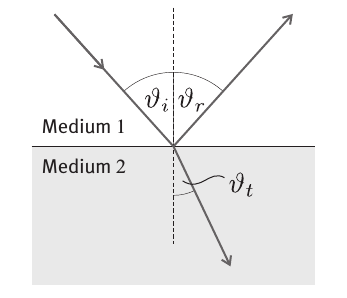
\includegraphics[width=0.4\linewidth]{./Bilder/Grenzschicht}
\caption{Brechung an Grenzfläche}
\label{fig:brech}
\end{figure}
Allgemein wird Licht immer in Richtung des optisch dichteren Mediums gebrochen.

\subsubsection{Brechung am Prisma}
Ein Lichtsstrahl wird am Prisma zweimal gebrochen. Das erste mal beim Einfallen, das zweite mal bei Ausfallen. Dadurch kommt es insgesamt zum Ablenkwinkel $ \delta $. Der minimale Ablenkwinkel $ \delta_m $ wird erreicht, wenn der Lichtstrahl das Prisma symmetrisch durchquert. Mit Innenwinkel $ \alpha $ des Prismas gilt für den Brechungsindex
\begin{equation}
	n = \frac{\sin \frac{\alpha + \delta_m}{2}}{\sin \delta_m} \label{eq:brech_pris}
\end{equation} 
Der Ablenkwinkel lässt sich, falls er nicht direkt messbar ist, auch mit
\begin{equation}
	\delta_m  = \arctan \frac{x_m}{y_m} \label{eq:delta}
\end{equation}
berechnen.

\subsubsection{Brechung an Linsen}
Linsen lassen sich in zwei Arten aufteilen. Es gibt zum einen Sammellinsen, welche kollimiertes, das heißt paralleles, Licht bündeln und Streulinsen, welche parallel einfallendes Licht streuen. Charakterisiert werden Linsen durch ihre Brennweite. Dies ist der Abstand zwischen Brennebene und Linsenebene. Die Brennebene ist die Ebene, in der alle Lichtstrahlen auf einen Punkt fokussiert werden. Im Fall einer Streulinse erhält man diese Ebene aus der gedachten Verlängerung des Lichtweges hinter der Linse und sie befindet sich vor der Linse.\\
Fällt das Licht nacheinander durch zwei Linsen der Brennweiten $ f_1 $ und $ f_2 $ mit Abstand $ d $, so ergeben die beiden Linsen ein Linsensystem mit Brennweite $ f $. Für diese gilt
\begin{equation}
	\frac{1}{f} = \frac{1}{f_1} + \frac{1}{f_2} - \frac{d}{f_1f_2}
\end{equation}
Im Fall $ d = f_1+f_2 $ gilt 
\begin{equation}
	\frac{1}{f} = \frac{1}{f_1} + \frac{1}{f_2} - \frac{f_1 + f_2}{f_1f_2} = 0
\end{equation}
und somit $ f = \infty $. Das heißt: Baut man ein Linsensystem, aus dem kollimiert einfallendes Licht auch kollimiert ausfällt, so lässt sich aus Brennweite der einen Linse und Abstand der Linsen die Brennweite einer unbekannten Linse bestimmen durch
\begin{equation}
	f_2 = d - f_1 \label{eq:linse}
\end{equation}

\subsubsection{Linsenfehler}
Bei Linsen können im wesentlichen drei Fehlerarten auftreten: chromatische Abberation, sphärische Abberation und Astigmatismus. Chromatische Abberation tritt bei monochromatischen Einfall nicht auf, und wird daher in diesem Versuch nicht betrachtet. \\
\textbf{Sphärische Abberation} tritt auf, wenn die Brennweite der Linse nach außen hin abnimmt. Weiter außen einfallendes Licht wird dann erst weiter von der Linse entfernt fokusiert als innen einfallendes Licht. Somit ergibt sich kein klarer Fokuspunkt mehr. \\
\textbf{Astigmatismus} tritt bei sphärischer Abberation im zweidimensionalen Fall auf. Durch die verschiedenen Brennweiten wird das Licht nicht gleichzeitig in $ x $- und $ y $-Richtung fokusiert. Daher ergibt sich kein Fokuspunkt, sondern ein Fokusstrich.

\subsection{Beugung am Gitter}
Fällt monochromatisches, kollimiertes Licht durch ein Gitter, so entstehen nach dem huygensschen Prinzip an jedem Gitterspalt Elementarwellen. Diese interferieren miteinander wobei der Gangunterschied winkelabhängig ist. Somit entsteht ein Interferenzmuster. Die Bedingung für Hauptmaxima in diesem ist
\begin{equation}
	\sin \theta_\mathrm{max} = m \frac{\lambda}{g}
\end{equation}
Dabei ist $ \vartheta_\mathrm{max} $ der Winkel der Maxima, $ m $ eine beliebige ganze Zahl, $ \lambda $ die Wellenlänge und $ g $ die Gitterkonstante.\\
Bestimmt man die Winkel unter denen die erstem Hauptmaxima auftreten, so ergibt sich aus der Dispersionsrelation 
\begin{equation}
	\lambda f = c_\mathrm M = \frac{c_0}{n}
\end{equation}
für das Verhältnis der Brechungsindizes
\begin{equation}
	\frac{n_1}{n_0} = \frac{\sin \vartheta_{\mathrm{max},0}}{\sin\vartheta_{\mathrm{max}, 1}} \label{eq:brech_wasser}
\end{equation}
\newpage
\section{Auswertung}
Die folgenden Versuche wurden mit zwei Lasern durchgeführt. Der im Folgenden als "roter Laser" bezeichnete Laser hat auf dem Gerät eine Wellenlänge von $\lambda = \SIrange{630}{680}{\nano\meter} $ angegeben. Der andere Laser, im Folgenden als "blauer Laser" bezeichnet, hat auf dem Gerät keine Wellenlänge angegeben. Daher wird die Angabe aus der Versuchsanleitung \cite[9]{anleitung2015} $ \lambda = \SI{405}{\nano\meter} $ angenommen.
\subsection{Brechung am Prisma}
In diesem Versuch wird der Brechungsindex eines Prismas aus Flintglas bestimmt. Dieser kann mit Hilfe von \eqref{eq:brech_pris} aus dem minimalen Ablenkungswinkel $ \delta_m $ und dem Innenwinkel des Prismenquerschnittes $ \alpha $ berechnet werden. Da das Prisma im Querschnitt ein gleichseitiges Dreieck ist, ist der Innenwinkel $ \alpha = \SI{60}{\degree} $. Um $ \delta_m $ zu bestimmen dreht man das Prisma so lange im Lichtstrahl, bis der Ablenkwinkel nicht mehr kleiner wird. Nun misst man die Abstände in $ x $- und $ y $-Richtung eines Punktes im Abgelenkten Strahl vom Prisma und erhält aus \eqref{eq:delta} den Ablenkwinkel. Dieser Versuch wird mit dem roten und dem blauen Laser durchgeführt. \\
Unsere Ergebnisse sind in Tabelle \ref{tab:prisma} zu finden. Die dazugehörigen Fehlerrechnungen \eqref{eq:err:delta} und \eqref{eq:err:npris} sind im Anhang zu finden.

\begin{table}[h]
\centering
\sisetup{table-figures-decimal = 1, table-figures-integer = 2, table-number-alignment = right, table-figures-uncertainty = 1}
\begin{tabular}{r|SSSS[table-figures-decimal = 3, table-figures-integer = 1]}
Laserfarbe & {$ x_m $ [\si{cm}]} & {$ y_m $ [\si{cm}]} 
& {$ \delta_m $ [\si{\degree}]} & {$ n $} \\\hline
rot & 58.0(5) & 54.0(5) & 47.0(4) & 1.608(4) \\
blau & 57.5(5) & 47.0(5) & 50.7(4) & 1.646(4)
\end{tabular}
\caption{Brechungsindex des Prismas}
\label{tab:prisma}
\end{table}


\subsection{Beugung am Gitter}
Das Ziel dieses Versuches ist es, den Brechungsindex von Wasser zu bestimmen. Dazu bestimmt man die Winkel der Hauptmaxima bei Beugung an einem Gitter mit Luft und mit Wasser als Medium. An einer Halbkreisküvette wird zunächst im leeren Zustand, also mit Luft als Medium, der Winkel der Hauptmaxima bestimmt. Daraufhin wird die Küvette mit Wasser gefüllt und man misst die Winkel der Hauptmaxima im Medium Wasser. Dies führt man mit dem roten und dem blauen Laser durch. Aus \eqref{eq:brech_wasser} erhält man dann das Verhältnis der Brechzahlen $ \frac{n_\mathrm{Wasser}}{n_\mathrm{Luft}} $ zwischen Wasser und Luft. Dieses entspricht nahezu dem Brechungsindex von Wasser, da der Brechungsindex der Luft nur minimal von dem des Vakuum abweicht. \\
Wir erhalten die Ergebnisse aus Tabelle \ref{tab:beug}. Die Fehler ergeben sich aus \eqref{eq:err:beug} im Anhang.
\begin{figure}[h]
	\centering
	\sisetup{table-figures-decimal = 1, table-figures-integer = 2, table-number-alignment = right, table-figures-uncertainty = 1}
	\begin{tabular}{r|SSS[table-figures-integer = 1, table-figures-decimal=2]}
	Laserfarbe & {$ \vartheta_\mathrm{max, Luft} $} & {$ \vartheta_\mathrm{max, Wasser} $} & $ \frac{n_\mathrm{Wasser}}{n_\mathrm{Luft}} $ \\\hline
	rot & 24.0(5) & 18.0(5) & 1.32(5) \\
	blau & 14.5(5) & 11.0(5) & 1.31(8)
	\end{tabular}
	\caption{Brechungsindex bei Beugungsversuch}
	\label{tab:beug}
\end{figure}

\subsection{Linsen}
Nun sollen zwei Linsen untersucht werden, eine Sammel- und eine Streulinse. Zunächst wird die Art der Linse bestimmt. Unsere Beobachtungen zeigen, dass die größere der beiden Linsen die Sammellinse und die kleinere der Linsen die Streulinse ist.
Das ist daran zu erkennen, dass beim durchgucken durch die Sammellinse das Bild auf dem Kopf steht und dies ist charakteristisch für Sammellinsen.
Außerdem ist das Bild, welches von der kleineren Linse erzeugt wird unscharf, was darauf schließen lässt, dass es sich um eine Streulinse handelt.
Für die Brennweite der Sammellinse wurde $ f=(9\pm1)\si{cm} $ gemessen. Das heißt, dass der fokussierte Strahl über 2cm Konstant fokussiert war.
Dieser Fehler ist relativ groß, die Gründe hierfür sind sowohl die Sphärische Aberration als auch der Linsenfehler.
Im nächsten Versuchsteil soll die Brennweite der Streulinse ermittelt werden, hierzu wird ein Linsensystem aus den beiden Linsen gebildet, welches den Laserstrahl kollimiert, das heißt, dass die Strahlen das System parallel verlassen.
Damit lässt sich die Gesamtbrennweite von $ f=\infty $ ableiten.
Der Abstand der Linsen von einander beträgt $ d=\SI{6\pm0,3}{cm} $ somit folgt mit \eqref{eq:linse}, $ f_{2}=d-f_{1} $ $ \Rightarrow $ $ f_{2}=\SI{-3\pm1.3}{cm} $, eine negative Brennweite ist für eine Streulinse charakteristisch.
Im letzten Aufgabenteil wird ein aufgeweiteter Lichtstrahl durch die Sammellinse geschickt, dabei wird der Strahl nicht mittig durch die Linse geschickt und die Linse wird gekippt.
Zunächst ist klar, dass falls der Strahl durch die Mitte geht, dieser fokussiert wird.
Wird der Strahl nun nicht mittig durch geschickt, so wird der Strahl ebenfalls fokussiert, aber zusätzlich wird dieser in die Richtung abgelenkt, in welche die Linse bewegt wurde.
Wird die Linse nun gekippt (sowohl Senkrecht als auch Horizontal) entstehen senkrechte Striche, es liegt also Astigmatismus vor.




\newpage
\section{Diskussion} 
\subsection{Demoversuch}
Im Demoversuch war zu beobachten, dass der Lichtstrahl eines grünen Lasers in einer Flüssigkeit nach unten gebogen wird. Qualitativ lässt sich das durch den Grundsatz der Optik erklären, dass Licht immer in Richtung des optisch dichteren Mediums abgelenkt wird. Quantitativ ließen sich mit dem Lagrange-Formalismus noch weitere Aussagen machen, jedoch wurden in diesem Versuch nur qualitative Beobachtungen gemacht.\\
Da der Lichtstrahl nach unten gekrümmt wird ist davon auszugehen das die Flüssigkeit nicht homogen, sondern im unteren Bereich des Beckens optisch dichter ist.  

\subsection{Ablenkung an Prisma}
In diesem Versuch ist die Wellenlängenabhängigkeit des Brechungsindex quantitativ gut nachgewiesen worden. Die Differenz der bestimmten Brechungsindizes liegt etwa eine Größenordnung über dem Fehler. Dies liegt insbesondere daran, dass der Versuch im Vergleich zur Einfachheit der Durchführung ein sehr genaues Ergebnis liefert. \\
Unsere Werte passen sehr gut in den Bereich $ n = \numrange{1.56}{1,93} $, welcher in der Literatur \cite{wiki:brechindex} für Flintglas angegeben ist.

\subsection{Beugung an Gitter}
Anhand der Beugung am Gitter ließen sich mit unseren Mitteln keine Wellenlängenabhängigkeit des Brechungsindex nachweisen. Die von uns ermittelten Werte liegen deutlich dichter bei einander als der systematische Fehler groß ist. Zudem liegen die Werte sehr nah am Literaturwert von $ n = \num{1.33} $ \cite{wiki:brechindex}. Es lässt sich aus unseren Ergebnissen nicht sagen, ob der Einfluss der Wellenlänge des Lichtes bei Wasser geringer ist als Flintglas, da eine Abweichung in der gleichen Größenordnung aufgrund der ungenaueren Messung durch den systematischen Fehler verschleiert werden könnte. \\
Der verhältnismäßig große Fehler ist hauptsächlich eine Folge der kleineren gemessenen Winkel. Wäre bei der Durchführung auch noch ein zweites oder drittes Hauptmaximum erkennbar gewesen, so hätte man die Winkel mit deutlich niedriger relativer Unsicherheit bestimmen können. Somit wäre auch der resultierende statistische Fehler geringer.

\subsection{Linsen}
Durch die Sphärische Aberration weist die Sammellinse einen relativ großen Bereich auf in dem der  Strahls konstant Fokussierung bleibt, somit ist die Brennweite nicht auf einen scharfen Punkt beschränkt sondern unscharf. Dies erlaubt keine genaue Bestimmung der Brennweite, welche sich auch auf die Unsicherheit der daraus abgeleiteten Werte auswirkt.
